\documentclass[12pt]{report}

\begin{document}
\chapter{Attuazione}

Il modulo di attuazione controlla l'uscita PWM per i servo-motori per guidare il braccio robotico lungo percorsi predefiniti.

Due input determinano il percorso da seguire e il punto corrente del percorso.

Altri input e output sono usati solo in fase di debug.

\section{Principio di funzionamento}

\begin{figure}
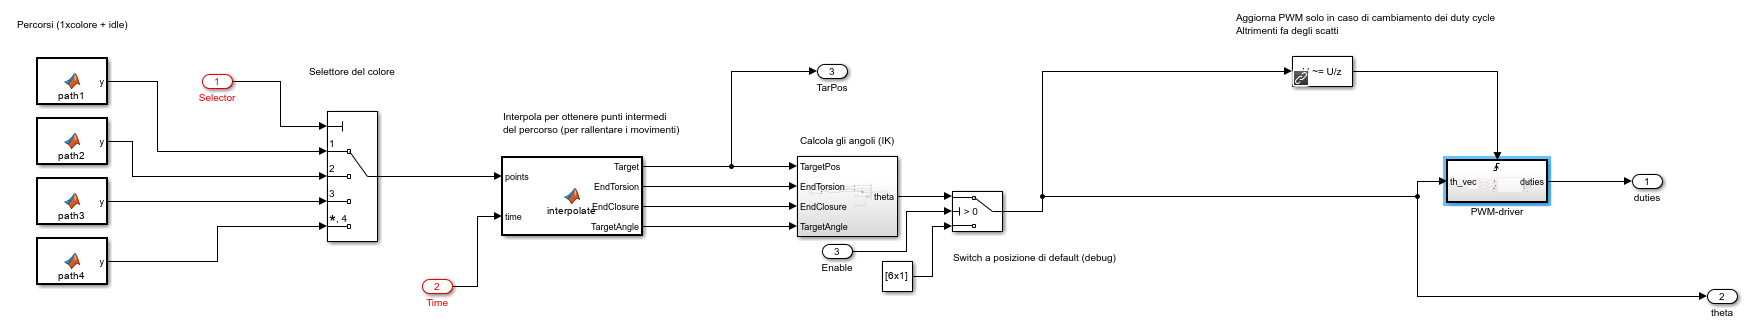
\includegraphics[width=\textwidth]{Complete_attuation}
\caption{Diagramma completo}
\end{figure}

I blocchi \textbf{Path1...Path4} restituiscono ognuno una matrice costante che rappresenta un percorso per il braccio robotico. Ogni riga rappresenta un punto chiave del percorso. A partire dai punti chiave vengono successivamete calcolati punti intermedi.

Ogni riga contiene 7 elementi:

\begin{itemize}
\item Distanza radiale in coordinate cilindriche dell'obiettivo dal centro della base del braccio robotico.
\item Angolo in cordinate cilindriche dell'obiettivo.
\item Distanza verticale in coordinate cilindriche dell'obiettivo dalla base del braccio robotico.
\item Angolo tra il vettore parallelo all'ultimo segmento del manipolatore (positivo verso la pinza) e la verticale (positiva verso l'alto).
\item Angolo del polso.
\item Angolo di chiusura della pinza.
\item Istante temporale del punto nel percorso.
\end{itemize}

\begin{figure}
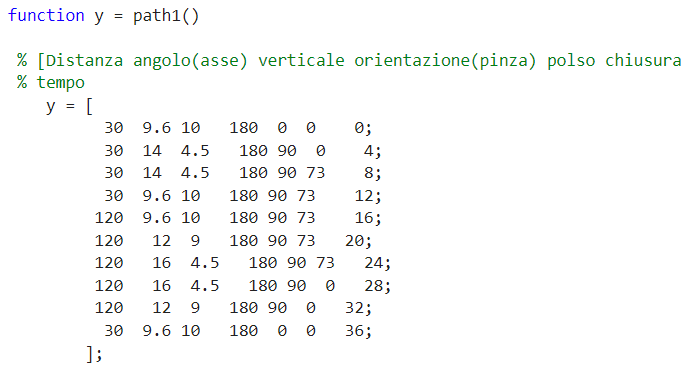
\includegraphics[width=\textwidth]{Path_structure}
\caption{Esempio di percorso}
\end{figure}

L'input \textbf{Selector} determina quale percorso verrà usato.

Il blocco \textbf{Interpolate} genera un punto intermedio interpolando linearmente due punti successivi nel percorso in base all'input \textbf{Time}.

Parte del blocco serve a garantire le corrette dimensioni della matrice in ingresso.

Vengono usati i punti estremi se \textbf{Time} eccede gli istanti temporali estremi.

Il blocco successivo calcola gli angoli dei servo-motori a partire dal punto interpolato.

Lo switch che segue permette di sostituire gli angoli calcolati con angoli predefiniti, per portare il manipolatore in una configurazione sicura durante il debug.

Il blocco \textbf{PWM-driver} imposta le uscite PWM a partire dagli angoli desiderati.

Questo blocco viene eseguito solo se gli angoli desiderati cambiano.

\section{Reimpostazione periodica del PWM}

Se il blocco \textbf{PWM-driver} venisse attivato liberamente (senza trigger al cambiamento) i servo-motori subirebbero uno scatto dovuto alla reimpostazione del PWM, che avviene anche quando i duty-cycle non variano.

Per questo è importante usare il blocco \textbf{Detect Change}. 

\section{Cinematica inversa}



\end{document}